% !TEX program = lualatex
\documentclass[10pt, leqno]{ltjsarticle}
% \documentclass[10pt]{ltjsarticle} % 日本語をそのまま扱えるクラス
% \usepackage[margin=28mm]{geometry}
\usepackage{amsmath,amssymb,mathtools}
\usepackage{amsthm}
\usepackage{tikz}
\usetikzlibrary{arrows.meta,positioning,calc}

\usepackage[
  top=15mm,     % 上余白
  bottom=15mm,  % 下余白
  left=10mm,    % 左余白
  right=10mm,    % 右余白
  landscape,
  margin=10mm
]{geometry}
% \usepackage[landscape,margin=20mm]{geometry} % 余白はお好みで
\usepackage{paracol}
\columnratio{0.5,0.5}             % 左右を 1:1 に
\setlength{\columnseprule}{0.4pt} % 真ん中の縦線

\usepackage{titlesec}
\titleformat{\paragraph}
  {\normalfont\bfseries}
  {}      % ← 番号を空に
  {0pt}
  {}

  % 左揃えディスプレイ用ブロック
\newcommand{\Tharray}[1]{%
  \[
  \begin{array}{@{}l@{}} % 余白なしで左端に揃える
    #1
  \end{array}
  \]
}
% 上線を楽に:\ov{X} = \overline{X}
\newcommand{\ov}[1]{\overline{#1}}
% --- 左揃えの Thボディ用ヘルパ (プリアンブル or 本文先頭に一度だけ )---
\newenvironment{Thleft}[1][]{%
  % \begin{theorem}[#1]\mbox{}\\[-1.25ex]\begingroup
  \begin{theorem}[#1]\mbox{}\\[0ex]\begingroup
  \setlength{\arraycolsep}{0pt}% 式中の余白をタイトに
  \renewcommand{\arraystretch}{1.0}% 行間
  \noindent$\begin{array}{@{}l@{}}%
}{%
  \end{array}$\par\endgroup\end{theorem}%
}


% ---- 記号・マクロ ----
\newcommand{\xto}{\mathrel{\xrightarrow{}}}
\newcommand{\into}{\hookrightarrow}
\newcommand{\epi}{\twoheadrightarrow}
\newcommand{\pto}{\rightrightarrows}
\newcommand{\cls}[1]{\bigl(#1\bigr)}
\newcommand{\redjoin}{\wedge}
\newcommand{\shrink}{\phi}
\newcommand{\Ex}{E}        % suspension functor E
\newcommand{\Ox}{\Omega}   % loop functor Omega
\newcommand{\id}{\mathrm{id}}
% --- Toda bracket helpers ---
\newcommand{\toda}[1]{\{\,#1\,\}}              % {a,b,c}
\newcommand{\todai}[2][]{\{\,#2\,\}_{#1}}      % {a,b,c}_i   (#1 は添字, 空なら無し) 
\newcommand{\todas}[1]{\langle\,#1\,\rangle}
\newcommand{\gen}[1]{\{#1\}}       % ⟨generator⟩ 表記を { } で統一
\newcommand{\Ker}{\operatorname{Ker}}
\newcommand{\im}{\operatorname{Im}}
\newcommand{\hs}[2]{\bigl[#1,#2\bigr]}   % 一般のホモトピー集合
\newcommand{\pis}[2]{\pi_{#1}(#2)}       % 左が球面のときのホモトピー群
\newcommand{\pit}[2]{\pi_{#1}^{#2}}
\newcommand{\ext}[1]{\overline{#1}}     % extension
\newcommand{\coext}[1]{\widetilde{#1}}  % coextension
\newcommand{\z}{\mathbb{Z}}
\newcommand{\sq}[1]{Sq^{#1}}

% ---- theorem-like environments ----
\numberwithin{equation}{section}
\theoremstyle{plain}
\newtheorem{theorem}{Theorem}[section]
\newtheorem{lemma}[theorem]{Lemma}
\newtheorem{proposition}[theorem]{Proposition}
\newtheorem{corollary}[theorem]{Corollary}
\theoremstyle{definition}
\newtheorem{definition}[theorem]{Definition}
\newtheorem{example}[]{Example}
\newtheorem{notation}[theorem]{Notation}
\newtheorem{assumption}[theorem]{Assumption}
\theoremstyle{remark}
\newtheorem{remark}[]{Remark}

% \title{PART 1 \quad CHAPTER I\\[2mm] General Composition and Secondary Composition}
\author{}
\date{}

\begin{document}

\setcounter{section}{8}

% ===== PART 2 / CHAPTER VIII p.82 =====
\section*{CHAPTER VIII\\Squaring Operations}

\begin{paracol}{2}

\[
\sq{i}:H^n(X;\z_2)\longrightarrow H^{n+i}(X;\z_2)
\]
を Steenrod の squaring operation とする.\\
Steenrod は, [18] の中で, functional squaring operation という準同型
\[
\pis{n+i-1}{S^n}\to\z_2
\] 
を与えた. 
この準同型を, 
\[
H_2:\ \pis{n+i-1}{S^n}\longrightarrow \z_2,\qquad (\,i>1\,)
\]
で表す. 
\(H_2\) は, 以下のように定義される. \\
\(\alpha\in \pis{n+i-1}{S^n}\) を取り, 
第I章で導入した cell 複体
\[
K_\alpha=S^n\cup_\alpha e^{n+i}
\]
を考える. 
これは up to homotopy で, 唯一つに定まる.
このとき,
\[
H_2(\alpha)\ne0\ (\mathrm{mod}\ 2)
\quad\Longleftrightarrow\quad
\sq{i}:\ H^n(K_\alpha;\z_2)\longrightarrow H^{n+i}(K_\alpha;\z_2)
\ \text{が同型}
\]
と定める.\\
\(i=1\) の場合, \(2\pis{n}{S^n}\) 上にも \(H_2\) を定義でき, 
\[
H_2:\ 2\pis{n}{S^n}\longrightarrow \z_2
\]
という準同型を得る. \\
\(Sq^1\) は係数群の完全列
\(0\to\z_2\to\z_4\to\z_2\to0\)
に関する Bockstein 準同型であることから, \\
次が容易に確かめられる.
\begin{equation}\label{eq:8.1}
H_2(2r\,\iota_n)\equiv r\pmod2, \qquad \text{for } r\in\z.
\end{equation}

\noindent
また, squaring operation の性質 ([Steenrod18]) から,
次が成り立つ.
\begin{equation}
% \noindent
% \textbf{(8.2).}\
\raisetag{4ex}
\begin{aligned}[t]
\text{i) }& H_2(\alpha)=0\quad \text{if }\ \alpha\in \pis{n+i-1}{S^n},\ i>n,\\
\text{ii) }& H_2\circ \Ex = H_2 .
\end{aligned}
\end{equation}
さらに, [1] により,
\(H_2\) は \(i=0,1,3,7\) 以外では, 自明であることが知られている.

\switchcolumn

\noindent
\cite{Steenrod1949}
N.~E.~Steenrod,
\newblock Cohomology invariants of mappings,
\newblock Ann. of Math., {\bf 50} (1949), 954--988.

\noindent
\textbf{Steenrod operantion の性質}\\
1).\ \(\sq{i}:H^n(X,A;\z_2)\to H^{n+i}(X,A;\z_2)\)
は natural transformation,\ \(n\ge0,\ i\ge0.\)\\
2).\ \(\sq{0} = 1.\)\\
3).\ \(\dim x = n\ \Longrightarrow\ \sq{n}x = x^2. \)\\
4).\ \(i>\dim x\ \Longrightarrow\ \sq{i}x = 0.\)\\
5).\ \textbf{Cartan formula:}\ 
\(\sq{k}(x y) = \sum_{i=0}^{k}\sq{i}x\cdot \sq{k-i}y.\)\\
6).\ \(\sq{1}\) は, 係数列 \(0\to\z_2\to\z_4\to\z_2\to0\) 
に関する Bockstein homomorphism.\\
7).\ \textbf{Adem relations:}\ 
\(\sq{a}\sq{b} = \sum_{j=0}^{[a/2]}\binom{b-1-j}{a-2j}
\sq{a+b-j}\sq{j},\ (0<a<2b)\).

\noindent
\cite{Adams1960}
J.~F.~Adams,
\newblock On the non-existence of elements of Hopf invariant one,
\newblock Ann. of Math., {\bf 72} (1960), 20--104.


\end{paracol}

\begin{paracol}{2}

\begin{proposition}
\(k=1, (3 \textnormal{ or } 7)\) とする. 
このとき,
\[
H_2:\ \pis{n+k}{S^n}\longrightarrow \z_2 \ : \ \textnormal{onto}
\quad\Longleftrightarrow\quad
n > k.
\]
\(n>k+1\) とすると, 
\[
H_2(\alpha)\not\equiv 0\ (\mathrm{mod}\ 2)
\quad\Longleftrightarrow\quad
\alpha\equiv
\begin{cases}
\eta_n,& k=1,\\
\nu_n, & k=3,\\
\sigma_n,& k=7,
\end{cases}
\mod 2\pis{n+k}{S^n},
\]
\(n=k+1\) とすると, 
\[
H_2(\alpha)\not\equiv 0\ (\mathrm{mod}\ 2)
\quad\Longleftrightarrow\quad
\alpha\equiv
\begin{cases}
\eta_2,& k=1,\\
\nu_4, & k=3,\\
\sigma_8,& k=7,
\end{cases}
\mod 2\pis{2k+1}{S^{k+1}} + E\pis{2k}{S^k}.
\]
\end{proposition}

% \switchcolumn

% \end{paracol}

% \begin{paracol}{2}

\noindent
\textbf{Proof.}\
複素数・四元数・Cayley 数の射影平面を考える. \\
これは, \(K_\alpha=S^{k+1}\cup_\alpha e^{2k+2}\) の形の cell 複体で, 
\(Sq^{k+1}\ne0\) を満たす. \\
この接着写像の類 \(\alpha\) は, Hopf class で, 
\(H_2(\alpha)\ne0\) である. 
よって,
\[
H_2:\ \pis{n+k}{S^n}\longrightarrow\z_2
\]
は, \(n=k+1\) のとき全射. \\
(8.2) ii) より,
\(H_2\) は \(n\ge k+1\) で全射.\\
(8.2) i) より,
\(H_2\) は \(n\le k\) では自明である. 
これで, 最初の主張が示せた. 

次に \(n>k+1\) の場合を考える. 
\(\pis{n+k}{S^n}\) は有限群であり, 
Prop 5.1, 5.6, 5.15 より,\\
\(\eta_n,\ \nu_n,\ \sigma_n\) (resp.) が
\(\pis{n+k}{S^n}\) の \(2\)-成分の生成元である. \\
\(H_2\) が全射なので, \(\Ker H_2 = 2\pis{n+k}{S^n}\) である.
したがって, 
\[
H_2(\alpha)\not\equiv0\pmod2
\quad\Longleftrightarrow\quad
\alpha\equiv
\eta_n\;(\nu_n, \ \sigma_n \text{ resp.})
\ \bmod\ 2\pis{n+k}{S^n}.
\]
最後に, \(n=k+1\) の場合を考える.\\
Hopf fibration により,
\(H(\beta)=\pm\iota_{2k+1}\) を満たす元 \(\beta\)
に対して,
\[
\pis{2k+1}{S^{k+1}}
\cong E\pis{2k}{S^k}\ \oplus\ \z\gen{\beta}.
\]
ここで, \(\beta\) は, 
\(H(\beta) = \pm\iota_{2k+1}\) を満たす任意の元を選んでよい.\\
そこで, \(\beta\) として, 
\(\eta_2,\ \nu_4,\ \sigma_8\) をそれそれ選ぶ.\\
(8.2) により, 
\(H_2(E\pi_{2k}(S^k)) = H_2(\pis{2k}{S^k}) = 0\) .\\
\(H_2\) が全射なので, 
\(H_2(\beta)\not\equiv0 \pmod2\) であり,\\
\(\Ker H_2 = 2\pis{2k+1}{S^{k+1}} + E\pis{2k}{S^k}\) である.
よって, 次が成り立つ.
\[
H_2(\alpha)\not\equiv 0 
\Longleftrightarrow
\alpha\equiv \beta \mod 2\pis{2k+1}{S^{k+1}} + E\pis{2k}{S^k} .
\]
\qed

\switchcolumn

\noindent
\textbf{(8.2).}\
\(\text{i) } H_2(\alpha)=0\quad \text{if }\ \alpha\in \pis{n+i-1}{S^n},\ i>n,\)\\
\(\text{ii) } H_2\circ \Ex = H_2 .\)\\
さらに, [1] により,
\(H_2\) は \(i=0,1,3,7\) 以外では, 自明であることが知られている.

\noindent
\textbf{Prop5.1.}\
\(\pi^{2}_{3}=\gen{\eta_2}\cong\mathbb Z,\quad
\pi^{n}_{n+1}=\gen{\eta_n}\cong\mathbb Z_2\ (n\ge3),\quad
(G_1;2)=\gen{\eta}\cong\mathbb Z_2.\) \\
ここで, 
\(H(\eta_2)=\iota_3,\ \Delta(\iota_5)=\pm 2\,\eta_3\) が成り立つ. 

\noindent
\textbf{Prop5.6.}\
\(\pi^{2}_{5}=\gen{\eta_{2}^{3}}\cong \mathbb Z_{2},\) \\
\(\pi^{3}_{6}=\gen{\nu'}\cong \mathbb Z_{4},\) \\
\(\pi^{4}_{7}=\gen{\nu_{4}}\oplus \gen{E\nu'}\cong \mathbb Z\oplus\mathbb Z_{4},\) \\
\(\pi^{n}_{n+3}=\gen{\nu_{n}}\cong \mathbb Z_{8}\ (n\ge5),\)\qquad
\((G_{3};2)=\gen{\nu}\cong \mathbb Z_{8}.\)

\noindent
\textbf{Prop5.15.}\
\(\pi_9^2=\pi_{10}^3=\pi_{11}^4=0,\) \\
\(\pi^{5}_{12}=\mathbb Z_2\gen{\sigma'''},\) \
\(\pi^{6}_{13}=\mathbb Z_4\gen{\sigma''},\) \
\(\pi^{7}_{14}=\mathbb Z_8\gen{\sigma'},\) \
\(\pi^{8}_{15}=\mathbb Z\gen{\sigma_8}\oplus\mathbb Z\gen{E\sigma'},\) \\
\(\pi^{n}_{n+7}=\mathbb Z_{16}\gen{\sigma_n}\ (n\ge9),\) \
\((G_{7};2)=\mathbb Z_{16}\gen{\sigma}.\)



\end{paracol}

\begin{paracol}{2}

\( \alpha\in\pi_n(X) \) を取り, 
Chapter I の空間
\[
X\cup_\alpha C S^n
\]
を考える. 
\(e^{n+1}\) を \(CS^n\) の内部, すなわち open \((n+1)\)-cell とし, 
\[
X\cup_\alpha C S^n = X\cup e^{n+1}
\]
と書く. 
\(p:X\cup e^{n+1}\to S^{n+1}\) を, (1.17) の shrinking map とする.
\[
u_{n+1}\in H^{n+1}(X\cup e^{n+1};\z_2)
\]
を, \(S^{n+1}\) の基本類の \(p^*\) による像とする. \\
今, \(\beta\in\pis{n+i-1}{S^n}\) を,
\(\alpha\circ\beta=0\) を満たすように取る.\\ 
coextension の定義により, 
\(\beta\) の coextension を表す写像
\[
f:S^{n+i}\longrightarrow X\cup_\alpha e^{n+1}
\]
を得る. 
(1.18) より, 合成 \(p\circ f\) は \(E\beta\) を表す. 


% ==== Chapter VIII p.84 ====

\begin{lemma}\label{lem:8.2}
% \noindent
% \textbf{Lem8.2.}\
$H_2(\beta)\ne0$ と仮定する. このとき,
\[
\sq{i}(u_{n+1}) = u_{n+i+1}
\quad\text{in} \ \ H^\ast (X\cup e^{n+1}\cup_f CS^{n+i}; \z_2).
\]
ここで, $u_{n+i+1}$ は $u_{n+1}$ と同様に, $CS^{n+i}$ により表される. 
\end{lemma}

\noindent
\textbf{Proof.}\
$X\subset X\cup e^{n+1}\cup_f CS^{n+1}$ 
の部分空間 \(X\) を一点につぶすことで, 
\[
p:\ X\cup e^{n+1}\cup_f CS^{n+i}\ \longrightarrow\ S^{n+1}\cup_{p\circ f} CS^{n+i}
\]
を得る. ここで, $H_2(E\beta)=H_2(\beta)\ne0$ なので, 
$S^{n+1}\cup_{p\circ f} CS^{n+i}$ において $Sq^i\ne0$ .
よって, 
\[
p^*: H^\ast(S^{n+1}\cup_{p\circ f}CS^{n+i};\z_2)
\ \longrightarrow\
H^\ast(X\cup e^{n+1}\cup_f CS^{n+i};\z_2)
\]
によって, $Sq^i\ u_{n+1}=u_{n+i+1}$ が成り立つ. 
\qed


以下では, この Lemma の使い方を, いくつかの例で示す. \\
ここでは, iterated squaring operantion における 
Adem's relations が本質的に有用である. 

\begin{example}
% \noindent
% \textbf{Example 1.}\
$H_2:\pis{n+k}{S^n}\to\z_2$ は,
$n\ge k+1$ かつ, $k=1,3,7$ で全射なので, \\
元 $\eta_n,\ \nu_n,\ \sigma_n$ は $2$ で割れず, 
よって, これらは 0 ではない. 
\end{example}

\switchcolumn

\noindent
\textbf{(1.17).}\
\(p:X\cup_\gamma CW\to EW,\
p(d'_W(w, t)) := d_W(w, t),\
p(X) := x_0.\)

\noindent
\(p^*: H^{n+1}(S^{n+1};\z_2)\to H^{n+1}(X\cup e^{n+1};\z_2)\).

\noindent
\textbf{(1.18).}\
\(p_*(\widetilde{\delta}) = E\delta,\
\widetilde{\delta}\in[EV, X\cup_\gamma CW]:\
\delta\in [V,W]\) の coextension.

\noindent
\textbf{(8.2).}\
\(\text{i) } H_2(\alpha)=0\quad \text{if }\ \alpha\in \pis{n+i-1}{S^n},\ i>n,\)\\
\(\text{ii) } H_2\circ \Ex = H_2 .\)\\
さらに, [1] により,
\(H_2\) は \(i=0,1,3,7\) 以外では, 自明であることが知られている.




\end{paracol}

\begin{paracol}{2}

\begin{example}
% \noindent
% \textbf{Example 2.}\
Toda bracket $\toda{2\iota_n,\ \eta_n,\ 2\iota_{n+1}}\not\equiv 0$．\\
$\pis{n+2}{S^n} = \z_2\gen{\eta_n^2}$ なので, 
$\toda{2\iota_n,\ \eta_n,\ 2\iota_{n+1}} = \gen{\eta_n^2}$. 
\end{example}

これを証明するために,
$0 \in \toda{2\iota_n,\ \eta_n,\ 2\iota_{n+1}}$ と仮定する.\\
\(K := S^n\cup_{\eta_n} e^{n+2}\) とすると, 
Prop 1.7 より, $2\iota_n$ の extension  $\alpha \in [K, S^n]$ と, \\
$2\iota_{n+1}$ の coextension  $\beta\in \pis{n+2}{K}$
が存在して, $\alpha\circ\beta=0$ を満たす.\\ 
$K$ において, $Sq^2\ne0$ が成り立つ. \\
さらに, $L := S^n\cup_\alpha CK = S^n\cup e^{n+1} \cup e^{n+3}$ とする.\\
\(S^n\cup e^{n+1}\) の接着写像は \(2\iota_n\) なので,
\(S^n\cup e^{n+1}\) の中で, \(\sq{1}\ne0\) である.\\
\(L\) の中で, \(\sq{2}\sq{1}\ne 0\) であることは容易にわかる.\\
\(\alpha\circ\beta = 0\) なので, 
\(\beta\) の coextension \(\coext{\beta} \in \pis{n+3}{L}\) が存在する.\\
\(
M := L\cup_{\coext{\beta}} CS^{n+3} = S^n\cup e^{n+1}\cup e^{n+3}\cup e^{n+4}
\)
とすると, \\
Lem \ref{lem:8.2}より, $M$ の中で $Sq^1 Sq^2 Sq^1 \ne 0$ である. \\
一方, Adem's relations から, $Sq^2 Sq^2 = Sq^1 Sq^2 Sq^1$.\\
$M$ に次元 $n+2$-cell が存在しないことから, 
\(M\) において $Sq^2 Sq^2 = 0$. \\
これは矛盾するので,
\(\toda{2\iota_n, \eta_n, 2\iota_{n+1}} \not\equiv 0\) である.
\qed

\switchcolumn

\noindent
\textbf{Prop1.7.}\
\(\todai[n]{\alpha, E^n\beta, E^n\gamma}
= (-1)^n\gen{\overline{\alpha}\circ E^n\widetilde{\gamma}}\).

\noindent
\textbf{Lem8.2.}\
$H_2(\beta)\ne0$ と仮定する. このとき,\\
\(
\sq{i}(u_{n+1}) = u_{n+i+1}
\quad\text{in} \ \ H^\ast (X\cup e^{n+1}\cup_f CS^{n+i}; \z_2).
\)\\
ここで, $u_{n+i+1}$ は $u_{n+1}$ と同様に, $CS^{n+i}$ により表される. 

\noindent
\textbf{Adem relations:}\ 
\(\sq{a}\sq{b} = \sum_{j=0}^{[a/2]}\binom{b-1-j}{a-2j}
\sq{a+b-j}\sq{j},\ (0<a<2b)\).



\end{paracol}

\begin{paracol}{2}

\begin{example}
% \noindent
% \textbf{Example 3.}\
$\eta_n^2, \nu_n^2, \eta_n\circ\sigma_{n+1}, \sigma_n^2$ は,
$2$ で割れず, \\
したがって, これらは自明ではない (Adem) . 
\end{example}

以下では, $\sigma_n^2$ の場合だけを示す (他の場合も同様) . \\
$\sigma_n^2=2\alpha,\ (\alpha\in\pis{n+14}{S^n})$ と仮定する. 
このとき,\\
\(
K = S^n\ \cup_{\sigma_n}\ e^{n+8}\ \cup_\alpha\ e^{n+15}\ \cup\ e^{n+16}
\)
において,\\
$e^{n+8}$ と $e^{n+15}$ はそれぞれ, $\sigma_n$ と $\alpha$
で接着され, \\
$e^{n+16}$ は, 
$\sigma_{n+7}-2\iota_{n+14}$ の coextension で接着されるとする. \\
$u_n,\ u_{n+8},\ u_{n+16}$ をそれぞれ, \\
$S^n,\ e^{n+8},\ e^{n+16}$ に対応する
$\mod 2$ コホモロジー類とすると, 
\[
\sq{8}\sq{8} u_n=\sq{8} u_{n+8}=u_{n+16}.
\]
一方, Adem's relations より,
\[
Sq^8 Sq^8 = Sq^{12} Sq^4 + Sq^{14} Sq^2 + Sq^{15} Sq^1 .
\]
明らかに,
\(\sq{1}u_n = \sq{2}u_n = \sq{4}u_n = 0\).\\
よって, $Sq^8 Sq^8 u_n = 0$ であるが, これは矛盾. 
したがって, $\sigma_n^2$ は $2$ で割れない.
\qed

\switchcolumn

\noindent
\(S^n\cup e^{n+8}\cup e^{n+15}
= S^n \cup _{\sigma_n\vee \alpha} C(S^{n+7}\vee S^{n+14})\),\\
\(S^n\xleftarrow{\sigma_n\vee\alpha}
S^{n+7}\vee S^{n+14}\xleftarrow{\sigma_{n+7}\vee -2\iota_{n+14}} S^{n+14}\),\\
\((\sigma_n\vee \alpha)\circ(\sigma_{n+7}\vee -2\iota_{n+14})
= \sigma_n^2\vee -2\alpha = 2\sigma_n^2 - 2\alpha = 0,\)\\
\(K = S^n\cup_{\sigma_n}e^{n+8}\cup_\alpha e^{n+15}
\cup_{\sigma_{n+7}-2\iota_{n+14}}e^{n+16}\).



\end{paracol}

\begin{paracol}{2}

% --- Example 4 ---
\begin{example}
% \noindent
% \textbf{Example 4.}\
次の Toda bracket の元
\[
\toda{\eta_n,\ \nu_{n+1},\ \eta_{n+4}},\quad
\toda{\nu_n,\ \eta_{n+3},\ \nu_{n+4}},\quad
\toda{\nu_n,\ \sigma_{n+3},\ \nu_{n+10}},\quad
\toda{\sigma_n,\ \nu_{n+7},\ \sigma_{n+10}}
\]
の元は, いずれも $2$ で割れない. したがって, これらは自明ではない. 
\end{example}

最後の Toda bracket の場合のみ示す (他も同様) . \\
$\alpha\in\pis{n+18}{S^n}$ が存在して,
$2\alpha\in \toda{\sigma_n,\ \nu_{n+7},\ \sigma_{n+10}}$
と仮定する. \\
$K=S^{n+7}\cup_{\nu_{n+7}}e^{n+11}$ 
とすると, Prop 1.7より, 
$\sigma_n$ の extension  $\beta\in [K, S^n]$ と,\\
$\sigma_{n+10}$ の coextension  $\gamma\in\pis{n+18}{K}$
が存在して, \(2\alpha = \beta\circ\gamma\) を満たす.
\[
F:=\beta\vee \alpha\ :K\vee S^{n+18}\to S^n,\qquad
G:=\gamma\vee(-2\iota_{n+18})\ : S^{n+18}\to K\vee S^{n+18}
\]
とすると,
\[
F\circ G= \beta\circ\gamma - \alpha\circ 2\iota_{n+18} = 0.
\]
Example2と同様に,
\[
L := S^n\cup_F C(K\vee S^{n+18})\ 
= \ S^n\cup e^{n+8}\cup e^{n+12}\cup e^{n+19}
\]
とし, $\lambda\in\pis{n+19}{L}$ を $G$ の coextension とする.
また, 
\[
M := L\cup_\lambda CS^{n+19}\simeq L\cup e^{n+20}
\]
とすると, 
$M$ において, $Sq^8 Sq^4 Sq^8 \ne 0$ が成り立つことが確かめられる. \\
一方, Adem's relation から,
\[
Sq^8 Sq^4 Sq^8 = Sq^4 Sq^{16} 
+ Sq^{16}Sq^4
+ (Sq^{18} + Sq^{14} Sq^4) Sq^2 + Sq^{15} Sq^4 Sq^1 .
\]
$M$ には, 
次元 $(n+1),(n+2),(n+4),(n+16)$ の cell が存在しないので, 右辺は $0$. \\
これは矛盾である. 
よって, $\toda{\sigma_n,\ \nu_{n+7},\ \sigma_{n+10}}$ の任意の元は
$2$ で割れない. 
\qed

% --- Lemma 8.3 (導入部)  ---

\bigskip
次に, operation \(\sq{16}\) について考える.
\begin{lemma}\label{lem:8.3}
% \noindent
% \textbf{Lem8.3.}\
$n\ge16$ とする. \\このとき,
\(
K=S^n\ \cup\ e^{n+8}\ \cup\ e^{n+16}
\)
なる \textnormal{cell} 複体が存在して, \\
$H^n(K;\z_2)$ の生成元 $u$ に対し,
\[
Sq^{16}u\ne0.
\]
ここで, 
\(e^{n+8}\) の接着写像は \(\sigma_n\) の,
\(e^{n+16}\) の接着写像は \(2\sigma_{n+7}\) の \textnormal{coextension} である.
\end{lemma}

\switchcolumn

\noindent
\textbf{Prop1.7.}\
\(\todai[n]{\alpha, E^n\beta, E^n\gamma}
= (-1)^n\gen{\overline{\alpha}\circ E^n\widetilde{\gamma}}\).

\noindent
\(S^n\xleftarrow{F = \beta\vee\alpha}
K\vee S^{n+18}\xleftarrow{G = \gamma\vee(-2\iota_{n+18})}S^{n+18},\
F\circ G = 0\).

\noindent
\(M = S^n\cup_{\sigma_n}e^{n+8}\cup_{\nu_{n+7}}e^{n+12}
\cup e^{n+19}\cup e^{n+20}\).

\noindent
\textbf{Adem relations:}\ 
\(\sq{a}\sq{b} = \sum_{j=0}^{[a/2]}\binom{b-1-j}{a-2j}
\sq{a+b-j}\sq{j},\ (0<a<2b)\).



\end{paracol}

\begin{paracol}{2}

\noindent
\textbf{Proof.}\
\(
M := S^8\cup_{\sigma_8} e^{16}
\)
とする. \\
$u_8,u_{16}$ を $S^8$ と $e^{16}$ に対応する $\mod 2$ コホモロジー類とすれば,
\[
Sq^8 u_8=u_{16}.
\]
Cartan の公式より, 
積空間 $M\times M$ において,
$Sq^{16}(u_8\times u_8) = u_{16}\times u_{16}$ である. \\
$M\wedge  M$ を考え, 
$\phi : M\times M\to M\wedge M$ を, 標準の shurinking map とする. \\
\[
M\wedge M = S^{16}\ \cup\ e^{24}_1\ \cup\ e^{24}_2\ \cup\ e^{32}
\]
であり,
\[
S^{16}\cup e^{24}_1 = M\wedge S^8 = E^8 M,\qquad
S^{16}\cup e^{24}_2\cup e^{32} = S^8 \wedge M.
\] 
$\mod2$ コホモロジーにおいて, \\
$S^{16},e^{32}$ はそれぞれ,
\(\phi^*\) によって, 
\(u_8\times u_8\) と $u_{16}\times u_{16}$ に写る.\\
よって, $Sq^{16}\neq0$ は $M\wedge M$ 上でも保たれる. \\
\(e_1^{24}, e_2^{24}\) の接着写像は, それぞれ, 
\(E^8\sigma_8 = \sigma_{16},\ \iota_8\wedge\sigma_8\) である.\\
Prop3.1 により,
\(\iota_8\wedge\sigma_8 = E^8\sigma_8 = \sigma_{16}\).\\
よって, 恒等写像 $\id_{S^{16}}$ の extension 
\[
f:\ S^{16}\cup e^{24}_2\longrightarrow S^{16}\cup e^{24}_1
\]
であって, $e^{24}_2$ を $e^{24}_1$ の上に, 次数 $1$ で写すものが存在する. \\
$e^{24}_2$ の各点を, $f$ での像と同一視すると, 次の cell 複体を得る：
\(
K=S^{16}\ \cup\ e^{24}\ \cup\ e^{32}.
\)\\
$K$ が, \(n=16\) に対する Lem \ref{lem:8.3} の条件を満たすことを示す. \\
\(M\wedge M\) から \(K\) への等化写像において, 
$S^{16}$ と $e^{32}$ は変化しない.\\
よって,
$Sq^{16}\neq0$ は \(K\) においても成り立つ. \\
さらに, $S^{16}\cup e^{24}= E^8M$ であるから, 
$e^{24}$ は \(S^{16}\) に $\sigma_{16}$ で接着されている. \\
次に, $e^{32}$ の接着写像を考える.\\
\(F:M\wedge M\to K\) 
を \(f\) による等化写像とする.\\
$p,p'$ をそれぞれ, $K$ と $M\wedge M$ における
$S^{16}$ をつぶす写像とする. \\
このとき, 次の図式を可換にする写像 $F'$ が存在する：
\[
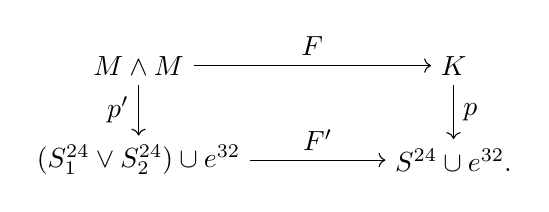
\begin{tikzpicture}[baseline=(current bounding box.center)]
\node (A) at (0,1.2) {$M\wedge M$};
\node (B) at (4,1.2) {$K$};
\node (C) at (0,0) {$(S^{24}_1\vee S^{24}_2)\cup e^{32}$};
\node (D) at (4,0) {$S^{24}\cup e^{32}.$};
\draw[->] (A) -- node[above] {$F$} (B);
\draw[->] (A) -- node[left] {$p'$} (C);
\draw[->] (B) -- node[right] {$p$} (D);
\draw[->] (C) -- node[above] {$F'$} (D);
\end{tikzpicture}
\]
ここで, $F'$ は $e^{32}$ を, 同相に $e^{32}$ の上に写し, 
$S^{24}_1,S^{24}_2$ を, 次数 $1$ で $S^{24}$ の上に写す. 

\switchcolumn

\noindent
\textbf{Lem8.3.}\
$n\ge16$ とする. \\
このとき,
\(
K=S^n\ \cup\ e^{n+8}\ \cup\ e^{n+16}
\)
なる \textnormal{cell} 複体が存在して, \\
$H^n(K;\z_2)$ の生成元 $u$ に対し,
\(
Sq^{16}u\ne0.
\)\\
ここで, 
\(e^{n+8}\) の接着写像は \(\sigma_n\) の,
\(e^{n+16}\) の接着写像は \(2\sigma_{n+7}\) の \textnormal{coextension} である.

\noindent
\textbf{Cartan formula:}\ 
\(\sq{k}(x y) = \sum_{i=0}^{k}\sq{i}x\cdot \sq{k-i}y.\)

\noindent
\textbf{Prop3.1.}\
\(
\alpha \wedge \beta
= (-1)^{(p+k)h} E^{q}\alpha \circ E^{p+k}\beta
= (-1)^{ph} E^{p}\beta \circ E^{q+h}\alpha .
\)



\end{paracol}

\begin{paracol}{2}

$L:=(S^{24}_1\vee S^{24}_2)\cup e^{32}$ とする.
このとき,
\[
L/S_1^{24} = S_2^{24}\cup_{E^{16}\sigma_8} e^{32} 
= S_2^{24} \cup_{\sigma_{24}} e^{32},
\]
\[
L/S_2^{24} = S_1^{24}\cup_{\iota_{16}\wedge\sigma_8} e^{32}
= S_1^{24} \cup_{\sigma_{24}}e^{32}.\ (\textnormal{Prop3.1})
\]

% ==== Chapter VIII p.87 ====

\noindent
以上の議論は, $S^{24}_1,S^{24}_2,e^{32}$ の向きを適切に選んで, \\
shurinking map が
向きを保存するようにしてあることに注意する. \\
$L$ における $e^{32}$ の接着写像の類は, \\
$M\wedge  S^{16}$ と $S^{16}\wedge  M$ における接着写像のクラスの和で表される.
写像 
\[
F' : (S_1^{24}\vee S_2^{24})\cup e^{32} \to S^{24}\cup e^{32}
\] 
により, $e^{32}$ の向きを適切に選べば, 
$e^{32}$ の接着写像のクラスは, $2\sigma_{24}$ となる.
\[
p_0 := p|_{S^{16}\cup e^{24}}\ : S^{16}\cup e^{24} \to S^{24}
\]
とし, 誘導準同型
\[
p_{0*}:\ \pi_{31}(S^{16}\cup e^{24})\ \longrightarrow\ \pi_{31}(S^{24})
\]
を考える. [6] のTh 2 により,
\[
p_{0*}:\pis{31}{S^{16}\cup e^{24}, S^{16}}
\xrightarrow{\cong} \pis{31}{S^{24}}.
\]
(1.18) より, 
\[
p_{0*}(\gamma)=2\sigma_{24}
\ \Longleftrightarrow\ \gamma \text{ は } 2\sigma_{23} \text{ の coextension.}
\]
したがって, $K$ における $e^{32}$ の接着写像は $\pm\gamma$ である. \\
必要ならば, $e^{32}$ の向きを変えることで, Lem は $n=16$ の場合について成立する. \\
$n>16$ の場合は, $\Ex^{\,n-16}K$ を考えることにより証明される. 
\qed

\begin{theorem}\label{thm:8.4}
% \noindent
% \textbf{Th8.4.}\
\end{theorem}
\(
\begin{array}{l}
\text{\rm i)\ \ Toda bracket  }
\toda{\sigma_n,\ 2\sigma_{n+7},\ \eta_{n+14}}
\text{ は, 次の形に分解できない元 } \alpha \text{ を含む. }\\
\qquad \qquad \qquad \alpha = 2\alpha' + \sum \beta_i\circ \gamma_i, \\
\qquad \text{ここで, } \alpha'\in \pis{n+16}{S^n},\
\beta_i\in \pis{n+k_i}{S^n},\ \gamma_i\in \pis{n+16}{S^{n+k_i}},\ 1<k_i<15.
\\[4pt]
\text{\rm ii)}\ \ \text{ Toda bracket  }\toda{\sigma_n,\ 2\sigma_{n+7},\ \nu_{n+14}}
\text{ は, 次の形に分解できない元 } \alpha \text{ を含む. }\\
\qquad \qquad \qquad \alpha = 2\alpha' + \sum \beta_i\circ \gamma_i, \\
\qquad \text{ここで, } \alpha'\in \pis{n+18}{S^n},\
\beta_i\in \pis{n+k_i}{S^n},\ \gamma_i\in \pis{n+18}{S^{n+k_i}},\\
\qquad 1<k_i<18,\ k_i\ne 3, 15.
\end{array}
\)

\switchcolumn

\noindent
\textbf{Lem8.3.}\
$n\ge16$ とする. \\
このとき,
\(K=S^n\ \cup\ e^{n+8}\ \cup\ e^{n+16}\)
なる \textnormal{cell} 複体が存在して, \\
$H^n(K;\z_2)$ の生成元 $u$ に対し,
\(Sq^{16}u\ne0.\)\\
ここで, 
\(e^{n+8}\) の接着写像は \(\sigma_n\) の,
\(e^{n+16}\) の接着写像は \(2\sigma_{n+7}\) の \textnormal{coextension} である.

\noindent
\cite{BlakersMassey1952}
A.~L.~Blakers and W.~S.~Massey,
\newblock The homotopy groups of a triad II,
\newblock Ann. of Math., {\bf 55} (1952), 192--201.

\noindent
\textbf{Th2.}\ \(\pi_i(X,A)=0\ (i<n),\ \pi_i(A)=0\ (i<m),\ 
p:(X,A)\to(X/A,*),\)\\
\(\Longrightarrow p_*:\pis{i}{X,A}\to\pis{i}{X/A}\)
は, \(i<n+m-1\) で同型. 
% \(\pis{i}{S^m_\infty, S^m_{p-1}}=0\ (i<pm),\ 
% \pis{i}{S^m_{p-1}} = 0\ (i<m).\)

\noindent
\textbf{(1.18).}\
\(p_*(\widetilde{\delta}) = E\delta,\qquad
\widetilde{\delta}\in[EV, X\cup_\gamma CW]:\
\delta\in [V,W]\) の coextension.




\end{paracol}

\begin{paracol}{2}

\noindent
\textbf{Proof.}\
i) を示す.  ii) の証明も同様である. \\
Lem 8.3 の複体
\(
K=S^n\cup e^{n+8}\cup e^{n+16}
\)
を考える. \\
$e^{n+16}$ の接着写像を,
\(
\delta\in \pis{n+15}{S^n\cup e^{n+8}}
\)
と置く. \\
Lem 8.3より, $\delta$ は $2\sigma_{n+7}$ の coextension である. \\
Prop 1.8により,  Toda bracket 
\(
\toda{\sigma_n,\ 2\sigma_{n+7},\ \eta_{n+14}}
\)
の中に,
\[
i_*(\alpha)\ =\ -\,\delta\circ\eta_{n+15}\ =\ \delta\circ\eta_{n+15}
\]
を満たす元 $\alpha$ が存在する.\\
% ==== Chapter VIII p.88 ====
\(
\alpha = 2\alpha' + \sum \beta_i\circ\gamma_i
\)
に分解できると仮定する. \\
\(S^n\cup_{\sigma_n}e^{n+8}\) に, 
$\alpha',\beta_i$ によって, cell を接着した cell 複体を $L_0$ とすると,\\
その \((n+2)\)-skeleton は \(S^n\) である.\\
仮定より, $\delta\circ\eta_{n+15}$ は,
\(
L = L_0\cup e^{n+16}
\)
において, 本質的でない. \\
したがって, $\eta_{n+15}$ の coextension 
\(
\delta'\in\pis{n+17}{L_0\cup_{\delta}e^{n+16}} = \pis{n+17}{L}
\)
が存在する. \\
\[
M := L \cup_{\delta'} e^{n+18}
  = L_0 \cup_{\delta} e^{n+16} \cup_{\delta'} e^{n+18}
\]
を考える. Lem 8.2より,
\(
Sq^2\,u_{n+16}=u_{n+18}
\)
が成り立つ. \\
$\delta\circ\eta_{n+15}$ の非本質性の中で,
\(
\alpha=2\alpha'+\sum \Ex\beta_i\circ\gamma_i
\)
という関係を用いる.\\
この関係式により, 
\(S^n\) の中で combine することと,\\
対応する cell に対する
$2\iota_{n+16}, \ \gamma_i$ の coextension を使うことにより, 
coextension \(\delta'\) を得る.\\
特に, $e^{n+18}$ は, 次数 $2$ で $e^{n+17}$ を cover しており, \\
この $e^{n+17}$ は, 唯一の $(n+17)$-cell で,
これは $\alpha'$ で接着されている. \\
したがって, \(u_{n+18}\neq0\) である. \\
また, $e^{n+16}$ は $M$ の唯一の $(n+16)$-cell なので, 
Lem 8.3より,
\[
Sq^2Sq^{16}\,u_n
 \ =\ Sq^2 u_{n+16}
 \ =\ u_{n+18}\ \neq\ 0 .
\]
一方, $L$ の $S^n$ を点に潰すと
\(
L/S^n
\)
を得るが, \\
これは
\(
K/S^n=S^{n+8}\cup_{2\sigma_{n+8}}e^{n+16}
\)
と, いくつかの球を一点でくっつけたものになる. 
\[
\begin{array}{lcl}
  L/S^n 
  & = & K/S^n\vee S^{n+17}\vee\cdots\vee S^{n+k_i+1}\vee\cdots\\
  & = & S^{n+8}\cup_{2\sigma_{n+8}}e^{n+16} \vee S^{n+17}\vee S^{n+k_i+1}\vee\cdots.  
\end{array}
\]
$K/S^n$ における squaring が自明であるから, 
$L/S^n$ における squaring も自明である.\\
よって, $a,b,c>0$ に対して,
\[
Sq^aSq^bSq^c=0
\quad\text{in } M=L\cup e^{n+18}.
\]

\switchcolumn

\noindent
\textbf{Th8.4.}\\
i).\ Toda bracket \(toda{\sigma_n,\ 2\sigma_{n+7},\ \eta_{n+14}}\)
は, 次の形に分解できない元 \(\alpha\) を含む. \\
\(\alpha = 2\alpha' + \sum \beta_i\circ \gamma_i,\) \\
ここで, \(\alpha'\in \pis{n+16}{S^n},\
\beta_i\in \pis{n+k_i}{S^n},\ \gamma_i\in \pis{n+16}{S^{n+k_i}},\ 1<k_i<15.\) \\
ii).\ Toda bracket \(\toda{\sigma_n,\ 2\sigma_{n+7},\ \nu_{n+14}}\)
は, 次の形に分解できない元 \(\alpha\) を含む. \\
\(\alpha = 2\alpha' + \sum \beta_i\circ \gamma_i,\) \\
ここで, \(\alpha'\in \pis{n+18}{S^n},\
\beta_i\in \pis{n+k_i}{S^n},\ \gamma_i\in \pis{n+18}{S^{n+k_i}},\)\\
\(1<k_i<18,\ k_i\ne 3, 15.\)

\noindent
\textbf{Lem8.3.}\
$n\ge16$ とする. \\
このとき,
\(K=S^n\ \cup\ e^{n+8}\ \cup\ e^{n+16}\)
なる \textnormal{cell} 複体が存在して, \\
$H^n(K;\z_2)$ の生成元 $u$ に対し,
\(Sq^{16}u\ne0.\)\\
ここで, 
\(e^{n+8}\) の接着写像は \(\sigma_n\) の,
\(e^{n+16}\) の接着写像は \(2\sigma_{n+7}\) の \textnormal{coextension} である.

\noindent
\textbf{(1.8).}\
\(d_n:S^n\times I\longrightarrow S^{n+1},\quad
d_n\bigl(\psi_n(t_1,\ldots,t_n),t\bigr)=\psi_{n+1}(t_1,\ldots,t_n,t).\)

\noindent
\textbf{Lem8.2.}\
$H_2(\beta)\ne0$ と仮定する. このとき,\\
\(
\sq{i}(u_{n+1}) = u_{n+i+1}
\quad\text{in} \ \ H^\ast (X\cup e^{n+1}\cup_f CS^{n+i}; \z_2).
\)\\
ここで, $u_{n+i+1}$ は $u_{n+1}$ と同様に, $CS^{n+i}$ により表される. 




\end{paracol}

\begin{paracol}{2}

\noindent
ここで, Adem's relation により,
\[
\begin{aligned}
Sq^2Sq^{16}
&=\ Sq^8Sq^2Sq^8
  + (Sq^2Sq^{12}+Sq^{13} Sq^1)Sq^4 \\
&\quad + (Sq^{16}+Sq^{15} Sq^1)Sq^2
  + (Sq^{15}Sq^2+Sq^{14}Sq^3+Sq^{13}Sq^4)Sq^1.
\end{aligned}
\]
$(n+2)$-cell が存在しないので,
\[
Sq^2Sq^{16}\,u_n=0.
\]
しかし, これは上で得た
\(
Sq^2Sq^{16}\,u_n\neq0
\)
に矛盾する. したがって,
\[
\alpha=2\alpha'+\sum \beta_i\circ\gamma_i
\]
の形への分解は不可能である.
\qed

Th \ref{thm:8.4} は i) で $k_i=1,15$, ii) で $k_i=3,15$ を許しても成立する. \\
というのも,
\(
\pis{n+16}{S^n}
\)
には $H_2\neq0$ を与える元が存在せず,\\
 (言い換えると,
$S^n\cup e^{n+16}$ で, $Sq^{16}\neq0$ となる複体は存在しない) からである. \\
ゆえに,
\(\toda{\sigma_n,2\sigma_{n+7},\eta_{n+14}}\)
および,
\(\toda{\sigma_n,2\sigma_{n+7},\nu_{n+14}}\)
の任意の元に対して, \\
Th \ref{thm:8.4} が成り立つ. 

\switchcolumn

\noindent
\textbf{Th8.4.}\\
i).\ Toda bracket \(toda{\sigma_n,\ 2\sigma_{n+7},\ \eta_{n+14}}\)
は, 次の形に分解できない元 \(\alpha\) を含む. \\
\(\alpha = 2\alpha' + \sum \beta_i\circ \gamma_i,\) \\
ここで, \(\alpha'\in \pis{n+16}{S^n},\
\beta_i\in \pis{n+k_i}{S^n},\ \gamma_i\in \pis{n+16}{S^{n+k_i}},\ 1<k_i<15.\) \\
ii).\ Toda bracket \(\toda{\sigma_n,\ 2\sigma_{n+7},\ \nu_{n+14}}\)
は, 次の形に分解できない元 \(\alpha\) を含む. \\
\(\alpha = 2\alpha' + \sum \beta_i\circ \gamma_i,\) \\
ここで, \(\alpha'\in \pis{n+18}{S^n},\
\beta_i\in \pis{n+k_i}{S^n},\ \gamma_i\in \pis{n+18}{S^{n+k_i}},\)\\
\(1<k_i<18,\ k_i\ne 3, 15.\)




\end{paracol}

\newpage

\begin{paracol}{2}

\renewcommand{\refname}{References}
\begin{thebibliography}{99}

\bibitem{Adams1960}
J.~F.~Adams,
\newblock On the non-existence of elements of Hopf invariant one,
\newblock Ann. of Math., {\bf 72} (1960), 20--104.

\bibitem{Adem}
J.~Adem,
\newblock The relations on Steenrod powers of cohomology classes,
\newblock Algebraic geometry and topology, Princeton.

\bibitem{Barratt1955}
M.~G.~Barratt,
\newblock Track groups I, II,
\newblock Proc. London Math. Soc., {\bf 5} (1955), 71--106, 285--329.

\bibitem{Barratt1961}
M.~G.~Barratt,
\newblock Note on a formula due to Toda,
\newblock Jour. London Math. Soc., {\bf 36} (1961), 95--96.

% 5
\bibitem{BarrattHilton1953}
M.~G.~Barratt and P.~J.~Hilton,
\newblock On join operations of homotopy groups,
\newblock Proc. London Math. Soc., {\bf 3} (1953), 430--445.

\bibitem{BlakersMassey1952}
A.~L.~Blakers and W.~S.~Massey,
\newblock The homotopy groups of a triad II,
\newblock Ann. of Math., {\bf 55} (1952), 192--201.

\bibitem{Freudenthal1937}
H.~Freudenthal,
\newblock Über die Klassen der Sphärenabbildungen,
\newblock Compos. Math., {\bf 5} (1937).

\bibitem{Hopf1935}
H.~Hopf,
\newblock Über die Abbildungen von Sphären auf Sphären niedriger Dimension,
\newblock Fund. Math., {\bf 25} (1935).

\bibitem{James1955}
I.~M.~James,
\newblock Reduced product spaces,
\newblock Ann. of Math., {\bf 62} (1955), 170--197.

% 10
\bibitem{James1956}
I.~M.~James,
\newblock Suspension triad of a sphere,
\newblock Ann. of Math., {\bf 63} (1956), 407--429.

\bibitem{James1958}
I.~M.~James,
\newblock The intrinsic join: A study of the homotopy groups of Stiefel manifold,
\newblock Proc. London Math. Soc., {\bf 8} (1958), 507--535.

\bibitem{Moore1953}
J.~C.~Moore,
\newblock Some applications of homology theory to homotopy problems,
\newblock Ann. of Math., {\bf 58} (1953), 325--350.

\bibitem{Serre1951}
J.-P.~Serre,
\newblock Homologie singulière des espaces fibrés,
\newblock Ann. of Math., {\bf 54} (1951), 425--505.

\bibitem{Serre1953a}
J.-P.~Serre,
\newblock Cohomologie modulo 2 des complexes d'Eilenberg-MacLane,
\newblock Comm. Math. Helv., {\bf 27} (1953), 198--231.

% 15
\bibitem{Serre1953b}
J.-P.~Serre,
\newblock Groups d'homotopie et classes groupes abéliens,
\newblock Ann. of Math., {\bf 58} (1953), 258--294.

\bibitem{Serre1953c}
J.-P.~Serre,
\newblock Quelques calculs de groupes d'homotopie,
\newblock Comptes Rendus Paris, {\bf 236} (1953), 2475--2477.

\bibitem{Steenrod1951}
N.~E.~Steenrod,
\newblock Topology of fibre bundles,
\newblock Princeton.

\bibitem{Steenrod1949}
N.~E.~Steenrod,
\newblock Cohomology invariants of mappings,
\newblock Ann. of Math., {\bf 50} (1949), 954--988.

\bibitem{Steenrod1953}
N.~E.~Steenrod,
\newblock Cyclic reduced powers of cohomology classes,
\newblock Proc. Nat. Acad. Sci. U.S.A., {\bf 39} (1953), 217--223.

% 20
\bibitem{Toda1952}
H.~Toda,
\newblock Generalized Whitehead products and homotopy groups of spheres,
\newblock Jour. of Inst. Poly. Osaka City Univ., {\bf 3} (1952), 43--82.

\bibitem{Toda1956}
H.~Toda,
\newblock On double suspension $E^2$,
\newblock Jour. of Inst. Poly. Osaka City Univ., {\bf 7} (1956), 103--145.

\bibitem{Toda1957}
H.~Toda,
\newblock Reduced join and Whitehead product,
\newblock Jour. of Inst. Poly. Osaka City Univ., {\bf 8} (1957), 15--30.

\bibitem{Toda1958a}
H.~Toda,
\newblock On exact sequences in Steenrod algebra mod 2,
\newblock Memoirs Univ. of Kyoto, {\bf 31} (1958), 33--64.

\bibitem{Toda1958b}
H.~Toda,
\newblock $p$-primary components of homotopy groups II. mod $p$ Hopf invariant,
\newblock Memoirs Univ. of Kyoto, {\bf 31} (1958), 143--160.

% 25
\bibitem{Toda1959}
H.~Toda,
\newblock $p$-primary components of homotopy groups IV. Compositions and toric constructions,
\newblock Memoirs Univ. of Kyoto, {\bf 32} (1959), 297--332.

\bibitem{Whitehead1950a}
G.~W.~Whitehead,
\newblock A generalization of the Hopf invariant,
\newblock Ann. of Math., {\bf 51} (1950), 192--237.

\bibitem{Whitehead1950b}
G.~W.~Whitehead,
\newblock The $(n+2)$nd homotopy group of the $n$-sphere,
\newblock Ann. of Math., {\bf 52} (1950), 245--247.

\bibitem{Whitehead1941}
J.~H.~C.~Whitehead,
\newblock On adding relations to homotopy groups,
\newblock Ann. of Math., {\bf 42} (1941), 409--428.

\bibitem{Whitehead1944}
J.~H.~C.~Whitehead,
\newblock On the groups $\pi_n(V_{m,n})$ and sphere bundles,
\newblock Proc. London Math. Soc., {\bf 48} (1944), 243--291.

\end{thebibliography}

\end{paracol}


\end{document}
